\documentclass{article}
\usepackage{tikz}

\begin{document}

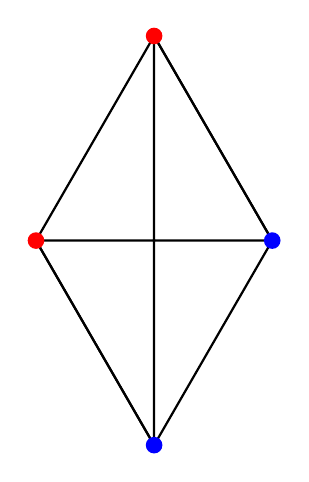
\begin{tikzpicture}[scale=1.5]
    % Define coordinates for the vertices
    \coordinate (A) at (0,0);
    \coordinate (B) at (2,0);
    \coordinate (C) at (1,1.732);
    \coordinate (D) at (1,-1.732);
    
    % Draw the outer diamond
    \draw[thick] (A) -- (B) -- (C) -- (D) -- cycle;
    
    % Draw the inner diamond
    \draw[thick] (A) -- (C) -- (B) -- (D) -- cycle;
    
    % Mark the vertices with colors
    \fill[red] (A) circle (2pt);
    \fill[blue] (B) circle (2pt);
    \fill[red] (C) circle (2pt);
    \fill[blue] (D) circle (2pt);
\end{tikzpicture}

\end{document}